\chapter{Organisasi atau Lingkungan Kerja Praktik}

\section{Struktur Organisasi}
Tuliskanlah struktur organisasi perusahaan KP dan jelaskan posisi tim KP pada struktur organisasi tersebut. Dalam gambar struktur organisasi, unit atau divisi tempat melaksanakan kerja praktik dibedakan dari unit lain dengan penambahan \textit{shading} atau garis putus-putus.

Perhatikan tata cara penggunaan gambar. Gambar yang Anda buat harus dijelaskan dalam paragraf sebelum gambar tersebut ditampilkan. Gambar~\ref{fig:komponen-dasar-sistem} menunjukkan sebuah gambaran umum dari suatu sistem yang terdiri dari masukan, proses, keluaran, dan umpan balik atau umpan ke depan.

\begin{figure}[H]
\centering
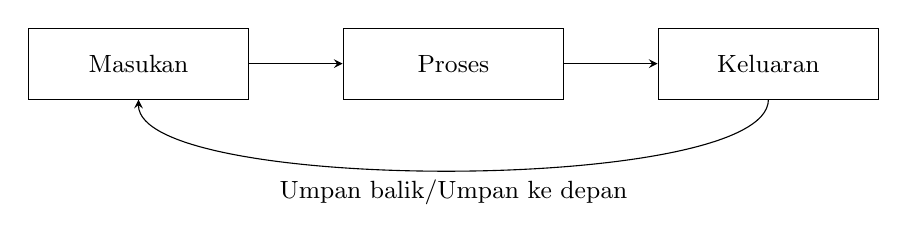
\begin{tikzpicture}[font=\small,>=stealth]
\node[draw,minimum width=2.8cm,minimum height=0.9cm] (a) at (0,0) {Masukan};
\node[draw,minimum width=2.8cm,minimum height=0.9cm] (b) at (4,0) {Proses};
\node[draw,minimum width=2.8cm,minimum height=0.9cm] (c) at (8,0) {Keluaran};
\draw[->] (a) -- (b);
\draw[->] (b) -- (c);
\draw[->] (c.south) .. controls +(0,-1.2) and +(0,-1.2) .. node[below]{Umpan balik/Umpan ke depan} (a.south);
\end{tikzpicture}
\caption{Komponen dasar sistem prediksi anomali pada stasiun pengawasan cuaca di Bandung (Kartodirjo 1977)}
\label{fig:komponen-dasar-sistem}
\end{figure}

Gambar yang Anda gunakan hendaknya merupakan gambar yang dibuat sendiri, bukan merupakan hasil \textit{copy-paste} dari sumber lain. Meskipun digambar sendiri, jika gambar tersebut diambil dari suatu sumber, tuliskan sumber referensinya seperti pada Gambar~\ref{fig:komponen-dasar-sistem}.

Istilah asing ditulis harus dalam huruf miring, misalnya pada penulisan \textit{copy-paste}. Jika ada istilah asing yang memiliki padanan dalam bahasa Indonesia, terjemahkan istilah tersebut ke dalam bahasa Indonesia, misalnya kata \textit{download} dapat diterjemahkan menjadi unduh.

Jika Anda ingin memerinci sesuatu, gunakan urutan dalam angka atau huruf seperti contoh berikut ini:
\begin{enumerate}[label=\arabic*)]
\item mewujudkan suatu produk;
\item memberikan arah dan pedoman dalam pelaksanaan kerja praktik; dan
\item mengoptimalkan pelaksanaan kerja praktik.
\end{enumerate}
Hindari penggunaan \textit{bullet point} dalam pemerincian.

\section{Unit Kerja}

\subsection{<Tambahkan Subbab Jika Diperlukan>}
Tuliskan lingkup pekerjaan divisi atau bagian tempat Anda melaksanakan KP secara ringkas. Kemudian, kaitkan lingkup pekerjaan divisi tersebut dengan lingkup pekerjaan Anda yang sesuai dengan lingkup dari divisi tersebut.

\subsection{<Tambahkan Subbab Jika Diperlukan>}
Untuk membuat tabel, Anda dibebaskan untuk membuat \textit{layout} tabel yang Anda inginkan. Perhatikan bahwa judul tabel ditulis di atas tabel dan diposisikan sedemikian rupa agar terlihat rapi. Tabel~\ref{tab:kelebihan-kekurangan} memperlihatkan contoh peletakan tabel.

\begin{table}[H]
\caption{Kelebihan dan kekurangan jenis-jenis soal ujian di kalangan sekolah menengah tingkat atas}
\label{tab:kelebihan-kekurangan}
\centering
\begin{tabularx}{\textwidth}{|p{3.2cm}|X|X|}
\hline
\textbf{Tipe} & \textbf{Kelebihan} & \textbf{Kekurangan} \\
\hline
Pilihan Ganda & Dapat menilai sesuatu & Cenderung hanya sesuatu \\
\hline
Benar-Salah & Menilai sesuatu & Sulit untuk melakukan sesuatu \\
\hline
Ujian Interpretasi & Dapat menilai sesuatu & Sulit untuk mengarahkan sesuatu \\
\hline
\end{tabularx}
\end{table}

\section{Deskripsi Pekerjaan}
Tuliskan deskripsi setiap tahap pekerjaan yang dilakukan dilengkapi dengan deskripsi pekerjaan mahasiswa KP terkait dengan organisasi tempat mahasiswa bekerja.

\section{Jadwal Kerja}
Tuliskan gambaran jadwal kegiatan selama KP, rinciannya mengacu ke lampiran \textit{Log Activity}.
